\section{Resultados}

\begin{frame}{Resultados}
    Experimentos são relizados com diferentes BRDFs para validar o compilador
   \begin{itemize}
       \item Metodologia padronizada:
             \begin{itemize}
                 \item O código fonte de entrada são equações no ambiente \texttt{equation} do \LaTeX{}
                 \item Tradução para GLSL pelo compilador desenvolvido neste trabalho
                 \item Visualização no Disney BRDF Explorer
             \end{itemize}
       \item Condições controladas:
             \begin{itemize}
                 \item Ângulos de luz fixos ($\theta_i = 33.89°$, $\phi_i = 145.83°$)
                 \item Gamma = 2.112, Exposição = -1.248
             \end{itemize}
   \end{itemize}
\end{frame}

\begin{frame}{Resultados: Experimentos}

\begin{itemize}
\item \textbf{11 Experimentos Realizados:}
    \begin{enumerate}
        \item Blinn-Phong
        \item Cook-Torrance
        \item Ward 
        \item Ashikhmin-Shirley
        \item Oren-Nayar 
        \item Cook-Torrance$_2$
        \item Ashikhmin-Shirley$_2$ 
        \item Dür
        \item Edwards-2006
        \item Kajiya-Kay-1989$_*$
        \item Minnaert
    \end{enumerate}
         % \begin{enum}
         %     \item Modelos Comuns:
         %     \item Modelos Avançados:
         %     \item Variações:
         %     \item Especializados/Outros:
         % \end{itemize}

\item Cada experimento ilustra:
         \begin{enumerate}
             \item Código fonte de entrada (\LaTeX{}) e saída (GLSL)
             \item Gráficos 3D e 2D de distribuição de reflexão
             \item Renderização de objetos 3D
         \end{enumerate}

    \end{itemize}
\end{frame}


%%%%%%%%%%%%%%%%%%%%%%%%%%%%%%%%%%%%%%%%%%%%%%%%%
% \subsection{Experimento Blinn-Phong}
%%%%%%%%%%%%%%%%%%%%%%%%%%%%%%%%%%%%%%%%%%%%%%%%%

\begin{frame}
\begin{figure}
    \frametitle{Experimento Blinn-Phong: Equações da BRDF em documento \LaTeX{}}
    \begin{center}
        % 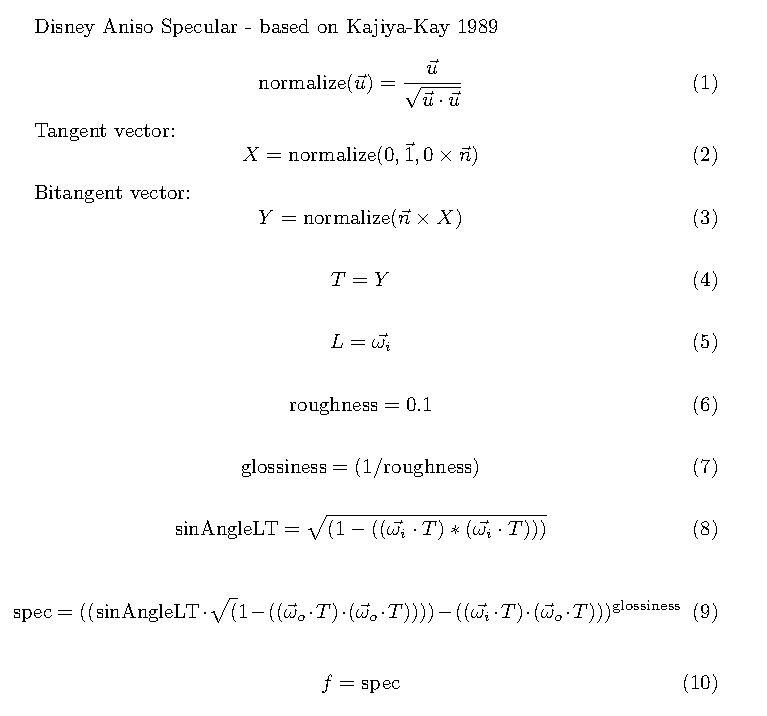
\includegraphics[scale=1.1,width=\textwidth]{./Imagens/brdfs/aniso.pdf}
        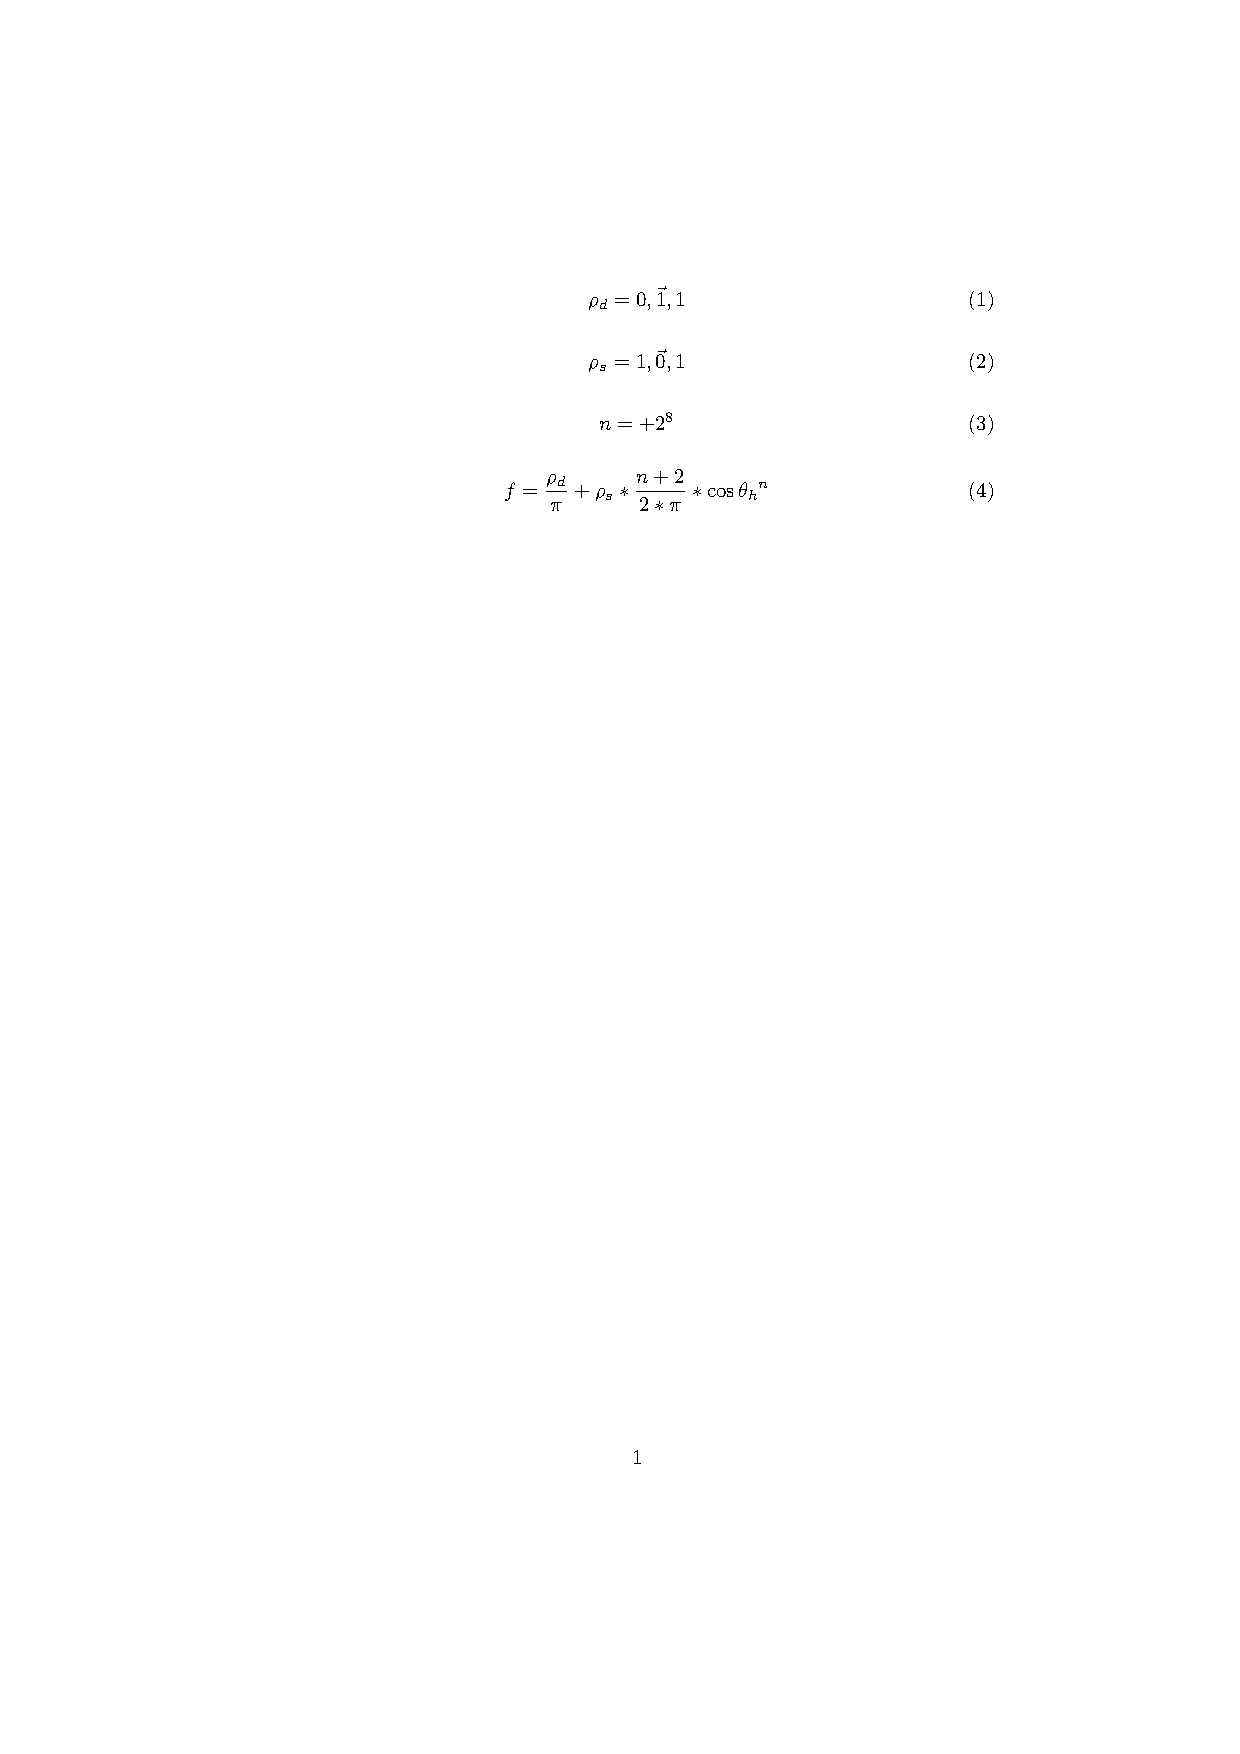
\includegraphics[scale=0.92]{./Imagens/brdfs/blinn-phong.pdf}
    \end{center}
\end{figure}
\end{frame}

%%%%%%%%%%%%%%%%%%%%%%%%%%%%%%%%%%%%%%%%%%%%%%%%%
\begin{frame}[fragile]
    \frametitle{Experimento Blinn-Phong: Código fonte \LaTeX{} da BRDF}
%%%%%%%%%%%%%%%%%%%%%%%%%%%%%%%%%%%%%%%%%%%%%%%%%
\begin{lstlisting}[language=tex, frame=none, inputencoding=utf8]
\begin{equation}
    \rho_{d} = \vec{0,1,1}
\end{equation}

\begin{equation}
    \rho_{s} = \vec{1,0,1}
\end{equation}

\begin{equation}
    n = +2^8
\end{equation}

\begin{equation}
f = \frac{\rho_{d}}{\pi} + \rho_{s} * \frac{n+2}{2*\pi} *
\cos{\theta_{h}}^{n}
\end{equation}
\end{lstlisting}
\end{frame}

\begin{frame}[fragile]
    \frametitle{Experimento Blinn-Phong: Código GLSL da BRDF deste experimento (1 de 2)}
\begin{clang}
analytic ::begin parameters
#[type][name][min val][max val][default val]
::end parameters
::begin shader
//////////// START OF BUILTINS DECLARTION ////////////
vec3 var_0_vec_h;
vec3 var_3_vec_n;
float var_10_theta_h;
float var_11_theta_d;
float var_1_pi;
float var_2_epsilon;
vec3 var_4_vec_omega_i;
float var_5_theta_i;
float var_6_phi_i;
vec3 var_7_vec_omega_o;
float var_8_theta_o;
float var_9_phi_o;
//////////// END OF BUILTINS DECLARTION ////////////
//////////// START OF USER DECLARED ////////////
vec3 var_12_rho_s;
float var_13_n;
vec3 var_14_rho_d;
vec3 var_15_f;
//////////// END OF USER DECLARED ////////////
\end{clang}
\end{frame}

\begin{frame}[fragile]
    \frametitle{Experimento Blinn-Phong: Código GLSL da BRDF deste experimento (2 de 2)}
\begin{clang}
vec3 BRDF(vec3 L, vec3 V, vec3 N, vec3 X, vec3 Y) {
  //////////// START OF BUILTINS INITIALIZATION ////////////
  var_0_vec_h = normalize(L + V);
  var_3_vec_n = normalize(N);
  var_1_pi = 3.141592653589793;
  var_2_epsilon = 1.192092896e-07;
  var_4_vec_omega_i = L;
  var_5_theta_i = atan(var_4_vec_omega_i.y, var_4_vec_omega_i.x);
  var_6_phi_i = atan(sqrt(var_4_vec_omega_i.y * var_4_vec_omega_i.y +
                          var_4_vec_omega_i.x * var_4_vec_omega_i.x),
                     var_4_vec_omega_i.z);
  var_7_vec_omega_o = V;
  var_8_theta_o = atan(var_7_vec_omega_o.y, var_7_vec_omega_o.x);
  var_9_phi_o = atan(sqrt(var_7_vec_omega_o.y * var_7_vec_omega_o.y +
                          var_7_vec_omega_o.x * var_7_vec_omega_o.x),
                     var_7_vec_omega_o.z);
  var_10_theta_h = acos(dot(var_0_vec_h, N));
  var_11_theta_d = acos(dot(var_0_vec_h, var_4_vec_omega_i));
  //////////// END OF BUILTINS INITIALIZATION ////////////
  var_12_rho_s = vec3(1.0, 0.0, 1.0);
  var_13_n = pow(2.0, 8.0);
  var_14_rho_d = vec3(0.0, 1.0, 1.0);
  var_15_f = ((var_14_rho_d / var_1_pi) +
              ((var_12_rho_s * ((var_13_n + 2.0) / (2.0 * var_1_pi))) *
               pow(cos(var_10_theta_h), var_13_n)));
  return vec3(var_15_f);
}
\end{clang}
\end{frame}

\begin{frame}{Experimento Blinn-Phong: Plots de Distruição de Reflexão}
\begin{figure}[H]
  
\caption{\small{\textit{Plots} da distribuição de reflexão especular e difusa do experimento Blinn-Phong.}}
    \label{fig-blinn-phong-plots}
\minipage{0.48\textwidth}
    \vspace{42px}
  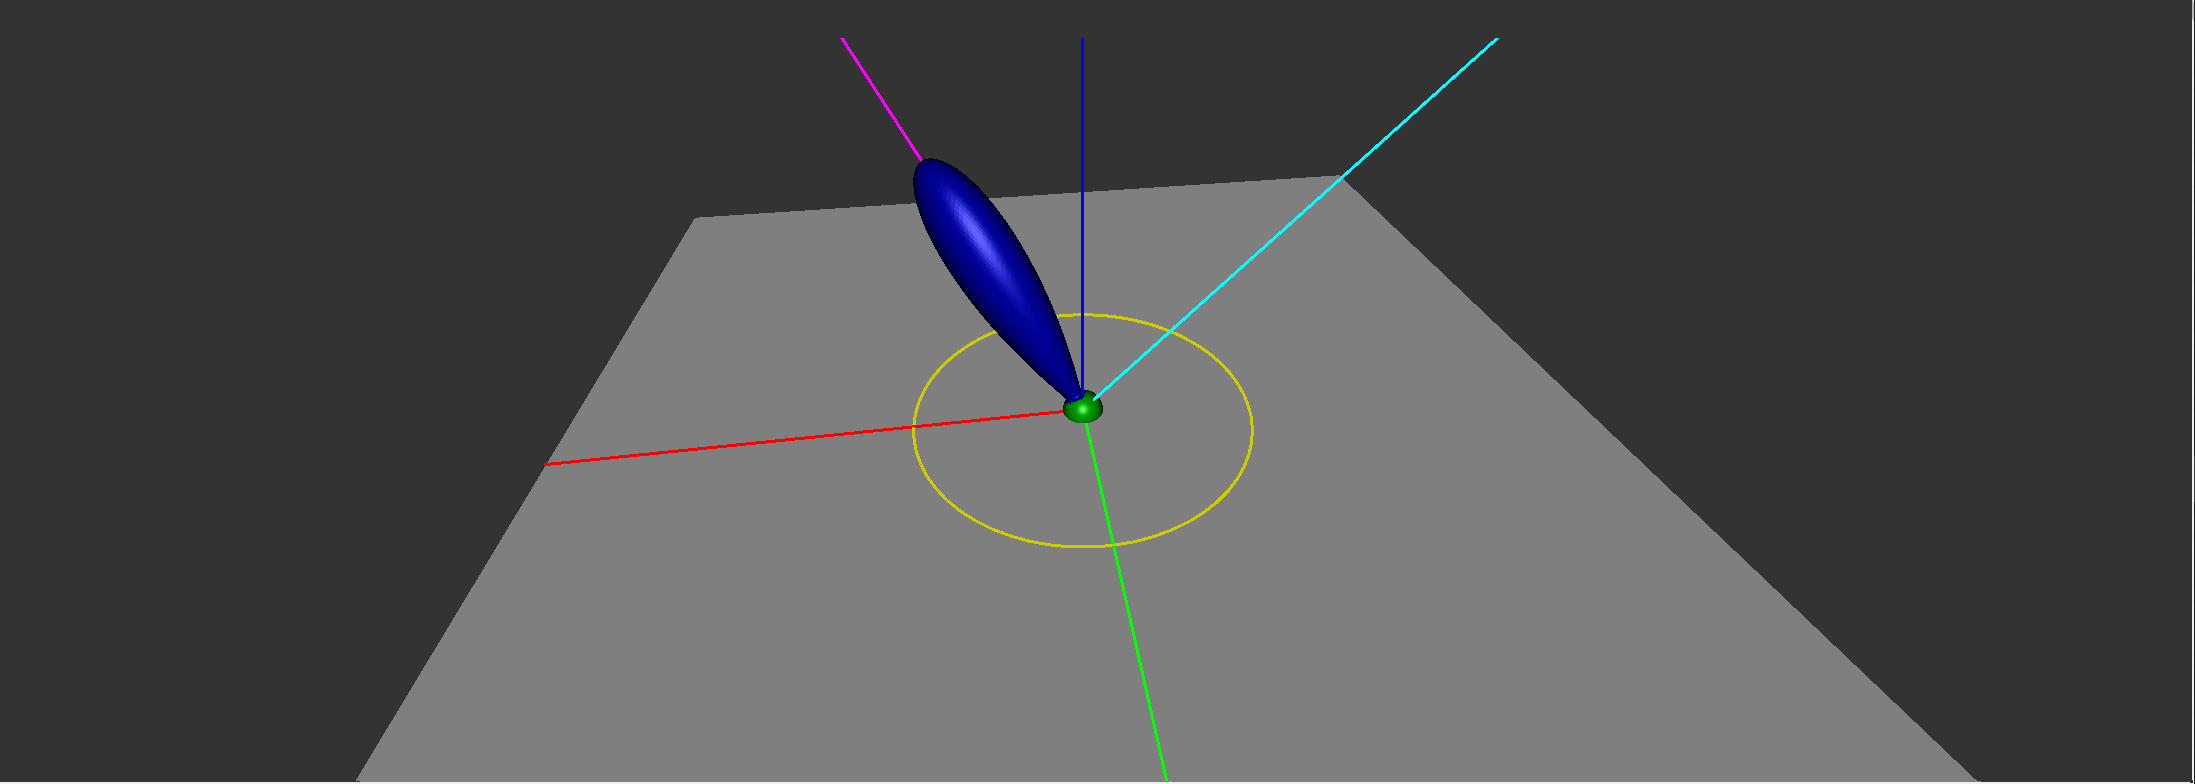
\includegraphics[width=\linewidth]{./Imagens/brdfs/blinn-phong-3D-plot}
    % \caption{\small{(a)}}\label{fig:awesome_image1}
    % \vspace{0.1px}
    % \legend{ \small (a) 3D \textit{plot}}
\endminipage\hfill
\minipage{0.48\textwidth}
  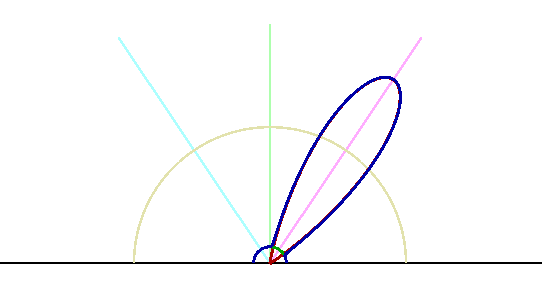
\includegraphics[width=\linewidth]{./Imagens/brdfs/blinn-phong-polar-plot-log.png}
    % \legend{ \small (b) \textit{Polar plot}}
    % \caption{\small{(b)}}\label{fig:awesome_image1}
\endminipage\hfill
\end{figure}
\end{frame}

\begin{frame}{Experimento Blinn-Phong: Objetos 3D renderizados para esta BRDF.}
\begin{figure}[H]
    \label{fig-blinn-phong-eqlang}
\minipage{0.32\textwidth}
  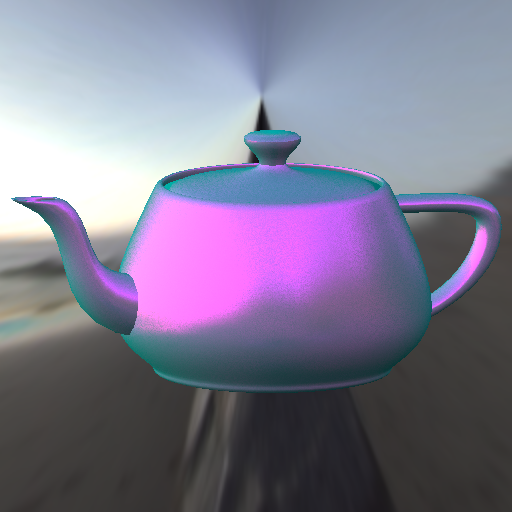
\includegraphics[width=\linewidth]{./Imagens/brdfs/blinn-phong-teapot.png}
    % \legend{ \small (a) \textit{Teapot}}
\endminipage\hfill
\minipage{0.32\textwidth}
  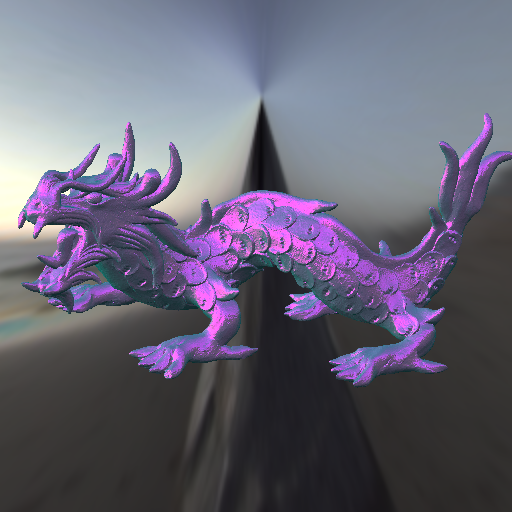
\includegraphics[width=\linewidth]{./Imagens/brdfs/blinn-phong-dragon.png}
    % \legend{ \small (b) Dragão de Stanford}
\endminipage\hfill
\minipage{0.32\textwidth}%
  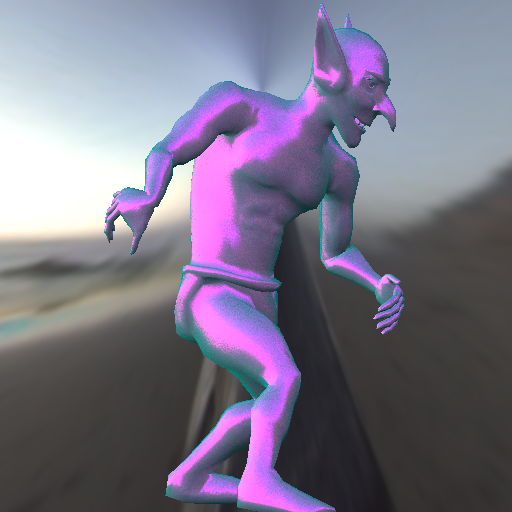
\includegraphics[width=\linewidth]{./Imagens/brdfs/blinn-phong-goblin.png}
    % \legend{ \small (c) Goblin}
\endminipage
\end{figure}
\end{frame}

%%%%%%%%%%%%%%%%%%%%%%%%%%%%%%%%%%%%%%%%%%%%%%%%%
% \subsection{Experimento Blinn-Phong}
%%%%%%%%%%%%%%%%%%%%%%%%%%%%%%%%%%%%%%%%%%%%%%%%%


%%%%%%%%%%%%%%%%%%%%%%%%%%%%%%%%%%%%%%%%%%%%%%%%%
% \subsection{Experimento Cook-Torrance}
%%%%%%%%%%%%%%%%%%%%%%%%%%%%%%%%%%%%%%%%%%%%%%%%%

\begin{frame}
\begin{figure}
    \frametitle{Experimento Cook-Torrance: Equações da BRDF em documento \LaTeX{}}
    \begin{center}
        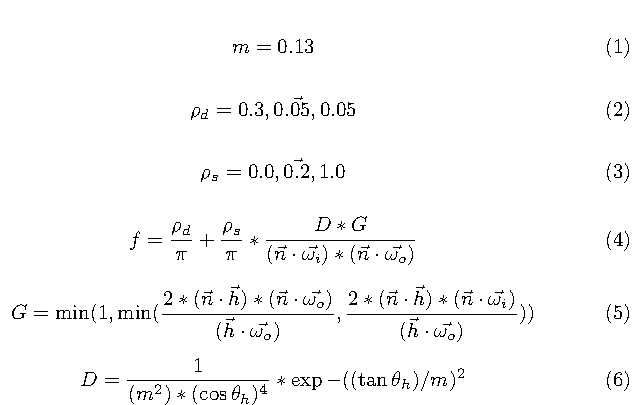
\includegraphics[scale=0.62]{./Imagens/brdfs/cook-torrance.pdf}
    \end{center}
\end{figure}
\end{frame}

%%%%%%%%%%%%%%%%%%%%%%%%%%%%%%%%%%%%%%%%%%%%%%%%%
\begin{frame}[fragile]
    \frametitle{Experimento Cook-Torrance: Código fonte \LaTeX{} da BRDF}
%%%%%%%%%%%%%%%%%%%%%%%%%%%%%%%%%%%%%%%%%%%%%%%%%
    \hspace{1cm}
\begin{lstlisting}[basicstyle=\ttfamily\scriptsize,language=tex, frame=none, inputencoding=utf8]
\begin{equation}
m = 0.13
\end{equation}

\begin{equation}
    \rho_{d} = \vec{0.3,0.05,0.05}
\end{equation}

\begin{equation}
    \rho_{s} = \vec{0.0,0.2,1.0}
\end{equation}

\begin{equation}
f = \frac{\rho_{d}}{\pi} + \frac{\rho_{s}}{\pi} *
\frac{D*G}{({\vec{n}}\cdot{\vec{\omega_{i}}}) *
({\vec{n}}\cdot{\vec{\omega_{o}}})}
\end{equation}

\begin{equation}
G = \min(1,\min( \frac{2 * ({\vec{n}}\cdot{\vec{h}}) * ({\vec{n}}\cdot{\vec{\omega_{o}}}) }
    {({\vec{h}}\cdot{\vec{\omega_{o}}})}, \frac{2 * ({\vec{n}}\cdot{\vec{h}}) *
({\vec{n}}\cdot{\vec{\omega_{i}}}) } {({\vec{h}}\cdot{\vec{\omega_{o}}})}))
\end{equation}

\begin{equation}
D = \frac{1} {(m^{2}) * (\cos{\theta_{h}})^{4}} * \exp{-((\tan{\theta_{h}})/m)^{2}}
\end{equation}
\end{lstlisting}
\end{frame}

\begin{frame}[fragile]
    \frametitle{Experimento Cook-Torrance: Código GLSL da BRDF deste experimento (1 de 2)}
\begin{clang}
analytic ::begin parameters
#[type][name][min val][max val][default val]
::end parameters
::begin shader
//////////// START OF BUILTINS DECLARTION ////////////
vec3 var_0_vec_h;
vec3 var_3_vec_n;
float var_10_theta_h;
float var_11_theta_d;
float var_1_pi;
float var_2_epsilon;
vec3 var_4_vec_omega_i;
float var_5_theta_i;
float var_6_phi_i;
vec3 var_7_vec_omega_o;
float var_8_theta_o;
float var_9_phi_o;
//////////// END OF BUILTINS DECLARTION ////////////
//////////// START OF USER DECLARED ////////////
float var_12_G;
vec3 var_13_rho_s;
float var_14_m;
float var_15_D;
vec3 var_16_rho_d;
vec3 var_17_f;
//////////// END OF USER DECLARED ////////////
//////////// START FUNCTIONS DECLARATIONS ////////////
//////////// END FUNCTIONS DECLARATIONS ////////////
\end{clang}
\end{frame}

\begin{frame}[fragile]
    \frametitle{Experimento Cook-Torrance: Código GLSL da BRDF deste experimento (2 de 2)}
\begin{clang}
vec3 BRDF(vec3 L, vec3 V, vec3 N, vec3 X, vec3 Y) {

  //////////// START OF BUILTINS INITIALIZATION ////////////
  var_0_vec_h = normalize(L + V);
  var_3_vec_n = normalize(N);
  var_1_pi = 3.141592653589793;
  var_2_epsilon = 1.192092896e-07;
  var_4_vec_omega_i = L;
  var_5_theta_i = atan(var_4_vec_omega_i.y, var_4_vec_omega_i.x);
  var_6_phi_i = atan(sqrt(var_4_vec_omega_i.y * var_4_vec_omega_i.y +
                          var_4_vec_omega_i.x * var_4_vec_omega_i.x), var_4_vec_omega_i.z);
  var_7_vec_omega_o = V;
  var_8_theta_o = atan(var_7_vec_omega_o.y, var_7_vec_omega_o.x);
  var_9_phi_o = atan(sqrt(var_7_vec_omega_o.y * var_7_vec_omega_o.y + var_7_vec_omega_o.x * var_7_vec_omega_o.x),
                     var_7_vec_omega_o.z);
  var_10_theta_h = acos(dot(var_0_vec_h, N));
  var_11_theta_d = acos(dot(var_0_vec_h, var_4_vec_omega_i));
  //////////// END OF BUILTINS INITIALIZATION ////////////

  var_12_G = min(1.0, min((((2.0 * (dot(var_3_vec_n, var_0_vec_h))) * (dot(var_3_vec_n, var_7_vec_omega_o))) / (dot(var_0_vec_h, var_7_vec_omega_o))), (((2.0 * (dot(var_3_vec_n, var_0_vec_h))) *
                            (dot(var_3_vec_n, var_4_vec_omega_i))) /
                           (dot(var_0_vec_h, var_7_vec_omega_o)))));
  var_13_rho_s = vec3(0.0, 0.2, 1.0);
  var_14_m = 0.13;
  var_15_D = ((1.0 / ((pow(var_14_m, 2.0)) * pow((cos(var_10_theta_h)), 4.0))) *
              exp((-pow((((tan(var_10_theta_h)) / var_14_m)), 2.0))));
  var_16_rho_d = vec3(0.3, 0.05, 0.05);
  var_17_f = ((var_16_rho_d / var_1_pi) + ((var_13_rho_s / var_1_pi) * ((var_15_D * var_12_G) / ((dot(var_3_vec_n, var_4_vec_omega_i)) * (dot(var_3_vec_n, var_7_vec_omega_o))))));
  return vec3(var_17_f);
}
\end{clang}
\end{frame}

\begin{frame}{Experimento Cook-Torrance: Plots de Distruição de Reflexão}
\begin{figure}[H]
  
\caption{\small{\textit{Plots} da distribuição de reflexão especular e difusa do experimento cook-torrance.}}
    \label{fig-cook-torrance-plots}
\minipage{0.48\textwidth}
    \vspace{42px}
  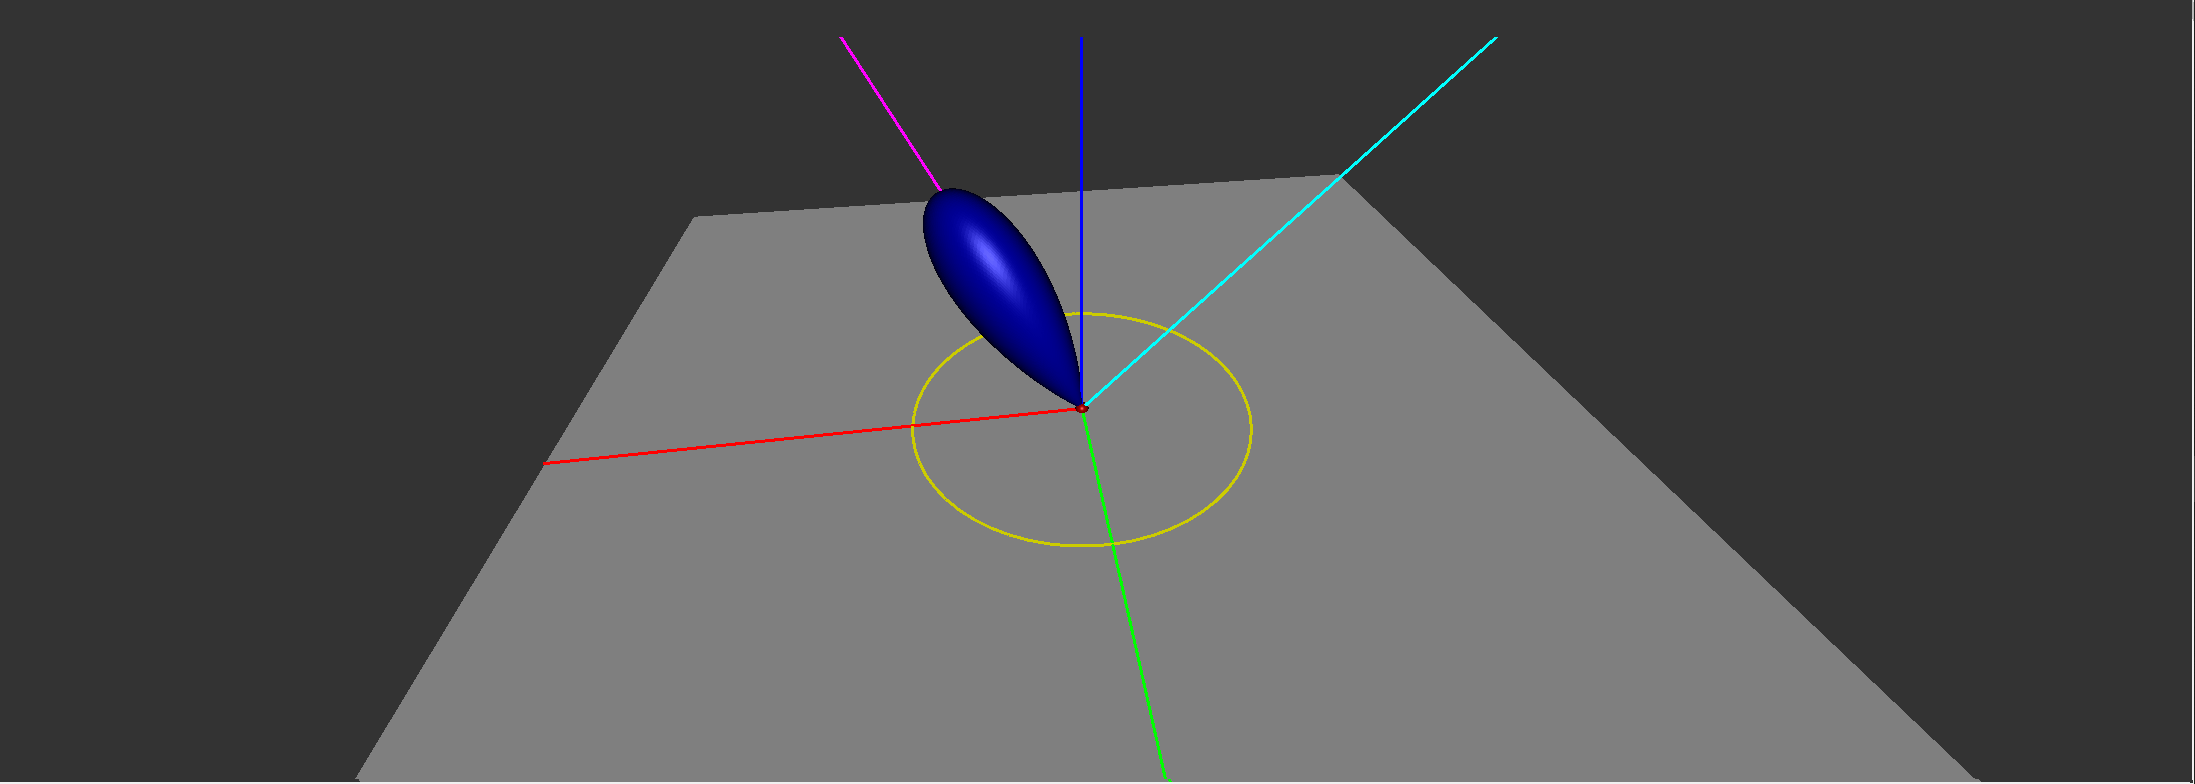
\includegraphics[width=\linewidth]{./Imagens/brdfs/cook-torrance-3D-plot}
    % \caption{\small{(a)}}\label{fig:awesome_image1}
    % \vspace{0.1px}
    % \legend{ \small (a) 3D \textit{plot}}
\endminipage\hfill
\minipage{0.48\textwidth}
  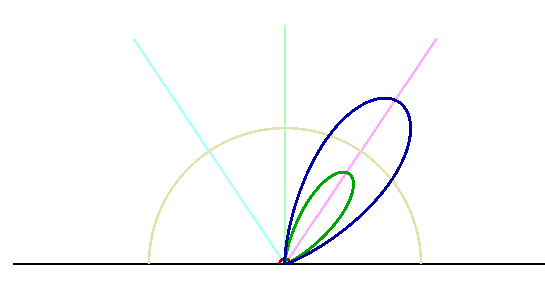
\includegraphics[width=\linewidth]{./Imagens/brdfs/cook-torrance-polar-plot-log.png}
    % \legend{ \small (b) \textit{Polar plot}}
    % \caption{\small{(b)}}\label{fig:awesome_image1}
\endminipage\hfill
\end{figure}
\end{frame}

\begin{frame}{Experimento Cook-Torrance: Objetos 3D renderizados para esta BRDF}
\begin{figure}[H]
    \label{fig-cook-torrance-eqlang}
\minipage{0.32\textwidth}
  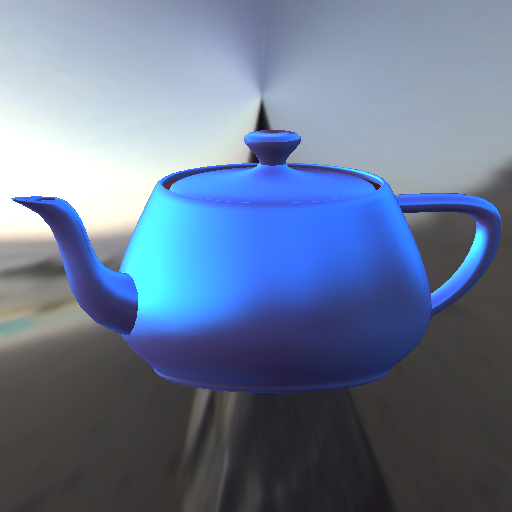
\includegraphics[width=\linewidth]{./Imagens/brdfs/cook-torrance-teapot.png}
    % \legend{ \small (a) \textit{Teapot}}
\endminipage\hfill
\minipage{0.32\textwidth}
  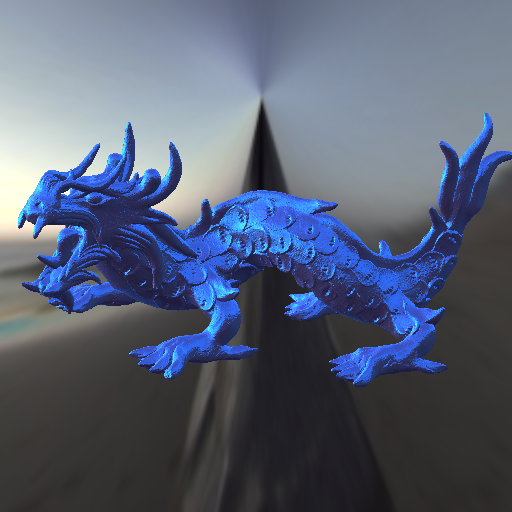
\includegraphics[width=\linewidth]{./Imagens/brdfs/cook-torrance-dragon.png}
    % \legend{ \small (b) Dragão de Stanford}
\endminipage\hfill
\minipage{0.32\textwidth}%
  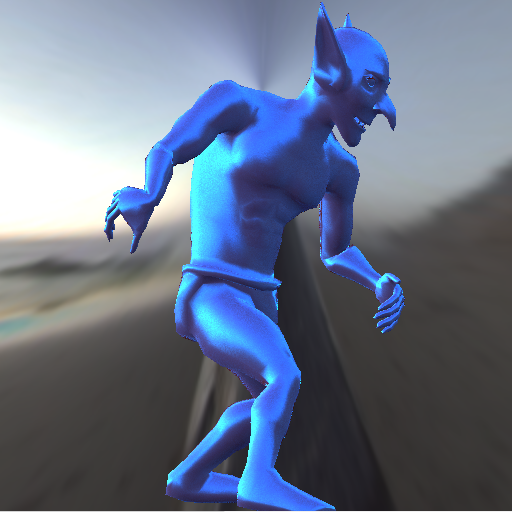
\includegraphics[width=\linewidth]{./Imagens/brdfs/cook-torrance-goblin.png}
    % \legend{ \small (c) Goblin}
\endminipage
\end{figure}
\end{frame}

%%%%%%%%%%%%%%%%%%%%%%%%%%%%%%%%%%%%%%%%%%%%%%%%%
% \subsection{Experimento Cook-Torrance}
%%%%%%%%%%%%%%%%%%%%%%%%%%%%%%%%%%%%%%%%%%%%%%%%%


%%%%%%%%%%%%%%%%%%%%%%%%%%%%%%%%%%%%%%%%%%%%%%%%%
% \subsection{Experimento Edwards-2006}
%%%%%%%%%%%%%%%%%%%%%%%%%%%%%%%%%%%%%%%%%%%%%%%%%

\begin{frame}
\begin{figure}
    \frametitle{Experimento Edwards-2006: Equações da BRDF em documento \LaTeX{}}
    \footnote{\tiny{Experimento adicionado aos slides para demonstrar definição de funções no formato $f(x,y) = x+y$.}}
    \begin{center}
        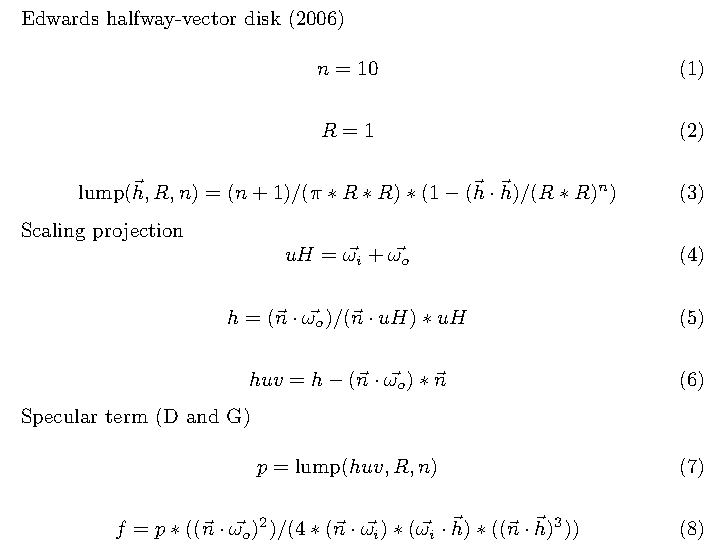
\includegraphics[scale=0.52]{./Imagens/brdfs/edwards-2006.pdf}
    \end{center}
\end{figure}
\end{frame}

%%%%%%%%%%%%%%%%%%%%%%%%%%%%%%%%%%%%%%%%%%%%%%%%%
\begin{frame}[fragile]
    \frametitle{Experimento Edwards-2006: Código fonte \LaTeX{} da BRDF}
%%%%%%%%%%%%%%%%%%%%%%%%%%%%%%%%%%%%%%%%%%%%%%%%%
    \vspace{-0.3cm}
    \hspace{2cm}
\begin{lstlisting}[basicstyle=\ttfamily\scriptsize,language=tex, frame=none, inputencoding=utf8]
\begin{equation}
n = 10
\end{equation}
\begin{equation}
R = 1
\end{equation}

\begin{equation}
\text{lump}(\vec{h}, R, n) = (n+1)/(\pi*R*R) * (1-(\vec{h} \cdot \vec{h})/(R*R)^ n)
\end{equation}

Scaling projection
\begin{equation}
    uH = \vec{\omega_i}+\vec{\omega_o} % // unnormalized H
\end{equation}
\begin{equation}
    h = (\vec{n} \cdot \vec{\omega_o}) / (\vec{n} \cdot uH) * uH
\end{equation}
\begin{equation}
    huv = h - (\vec{n} \cdot \vec{\omega_o}) * \vec{n}
\end{equation}
Specular term (D and G)
\begin{equation}
    p = \text{lump}(huv, R, n)
\end{equation}
\begin{equation}
    f = p * ((\vec{n} \cdot \vec{\omega_o})^ 2)
    / (4 * (\vec{n} \cdot \vec{\omega_i})
    * (\vec{\omega_i} \cdot \vec{h}) * ((\vec{n} \cdot \vec{h})^ 3))
\end{equation}
\end{lstlisting}
\end{frame}

\begin{frame}[fragile]
    \frametitle{Experimento Edwards-2006: Código GLSL da BRDF deste experimento (1 de 2)}
\begin{clang}
analytic ::begin parameters
#[type][name][min val][max val][default val]
::end parameters
::begin shader
//////////// START OF BUILTINS DECLARTION ////////////
vec3 var_0_vec_h;
vec3 var_3_vec_n;
float var_10_theta_h;
float var_11_theta_d;
float var_1_pi;
float var_2_epsilon;
vec3 var_4_vec_omega_i;
float var_5_theta_i;
float var_6_phi_i;
vec3 var_7_vec_omega_o;
float var_8_theta_o;
float var_9_phi_o;
//////////// END OF BUILTINS DECLARTION ////////////
//////////// START OF USER DECLARED ////////////
vec3 var_15_uH;
vec3 var_16_h;
float var_14_n;
vec3 var_17_huv;
float var_13_R;
float var_18_p;
float var_19_f;
//////////// END OF USER DECLARED ////////////
//////////// START FUNCTIONS DECLARATIONS ////////////
float var_12_text_lump(vec3 var_0_vec_h, float var_13_R, float var_14_n) {
  return ((((var_14_n + 1.0)) / (((var_1_pi * var_13_R) * var_13_R))) *
          ((1.0 - ((dot(var_0_vec_h, var_0_vec_h)) /
                   pow(((var_13_R * var_13_R)), var_14_n)))));
}
\end{clang}
\end{frame}

\begin{frame}[fragile]
    \frametitle{Experimento Edwards-2006: Código GLSL da BRDF deste experimento (2 de 2)}
\begin{clang}
//////////// END FUNCTIONS DECLARATIONS ////////////
vec3 BRDF(vec3 L, vec3 V, vec3 N, vec3 X, vec3 Y) {
  //////////// START OF BUILTINS INITIALIZATION ////////////
  var_0_vec_h = normalize(L + V);
  var_3_vec_n = normalize(N);
  var_1_pi = 3.141592653589793;
  var_2_epsilon = 1.192092896e-07;
  var_4_vec_omega_i = L;
  var_5_theta_i = atan(var_4_vec_omega_i.y, var_4_vec_omega_i.x);
  var_6_phi_i = atan(sqrt(var_4_vec_omega_i.y * var_4_vec_omega_i.y +
                          var_4_vec_omega_i.x * var_4_vec_omega_i.x), var_4_vec_omega_i.z);
  var_7_vec_omega_o = V;
  var_8_theta_o = atan(var_7_vec_omega_o.y, var_7_vec_omega_o.x);
  var_9_phi_o = atan(sqrt(var_7_vec_omega_o.y * var_7_vec_omega_o.y +
                          var_7_vec_omega_o.x * var_7_vec_omega_o.x), var_7_vec_omega_o.z);
  var_10_theta_h = acos(dot(var_0_vec_h, N));
  var_11_theta_d = acos(dot(var_0_vec_h, var_4_vec_omega_i));
  //////////// END OF BUILTINS INITIALIZATION ////////////
  var_15_uH = (var_4_vec_omega_i + var_7_vec_omega_o);
  var_16_h = (((dot(var_3_vec_n, var_7_vec_omega_o)) /
    (dot(var_3_vec_n, var_15_uH))) * var_15_uH);
  var_14_n = 10.0;
  var_17_huv = (var_16_h - ((dot(var_3_vec_n, var_7_vec_omega_o)) * var_3_vec_n));
  var_13_R = 1.0;
  var_18_p = var_12_text_lump(var_17_huv, var_13_R, var_14_n);
  var_19_f = ((var_18_p * (pow((dot(var_3_vec_n, var_7_vec_omega_o)), 2.0))) /
              ((((4.0 * (dot(var_3_vec_n, var_4_vec_omega_i))) *
                 (dot(var_4_vec_omega_i, var_0_vec_h))) * (pow((dot(var_3_vec_n, var_0_vec_h)), 3.0)))));
  return vec3(var_19_f);
}
\end{clang}
\end{frame}

\begin{frame}{Experimento Edwards-2006: Plots de Distruição de Reflexão}
\begin{figure}[H]
  
\caption{\small{\textit{Plots} da distribuição de reflexão especular e difusa do experimento edwards-2006.}}
    \label{fig-edwards-2006-plots}
\minipage{0.48\textwidth}
    \vspace{42px}
  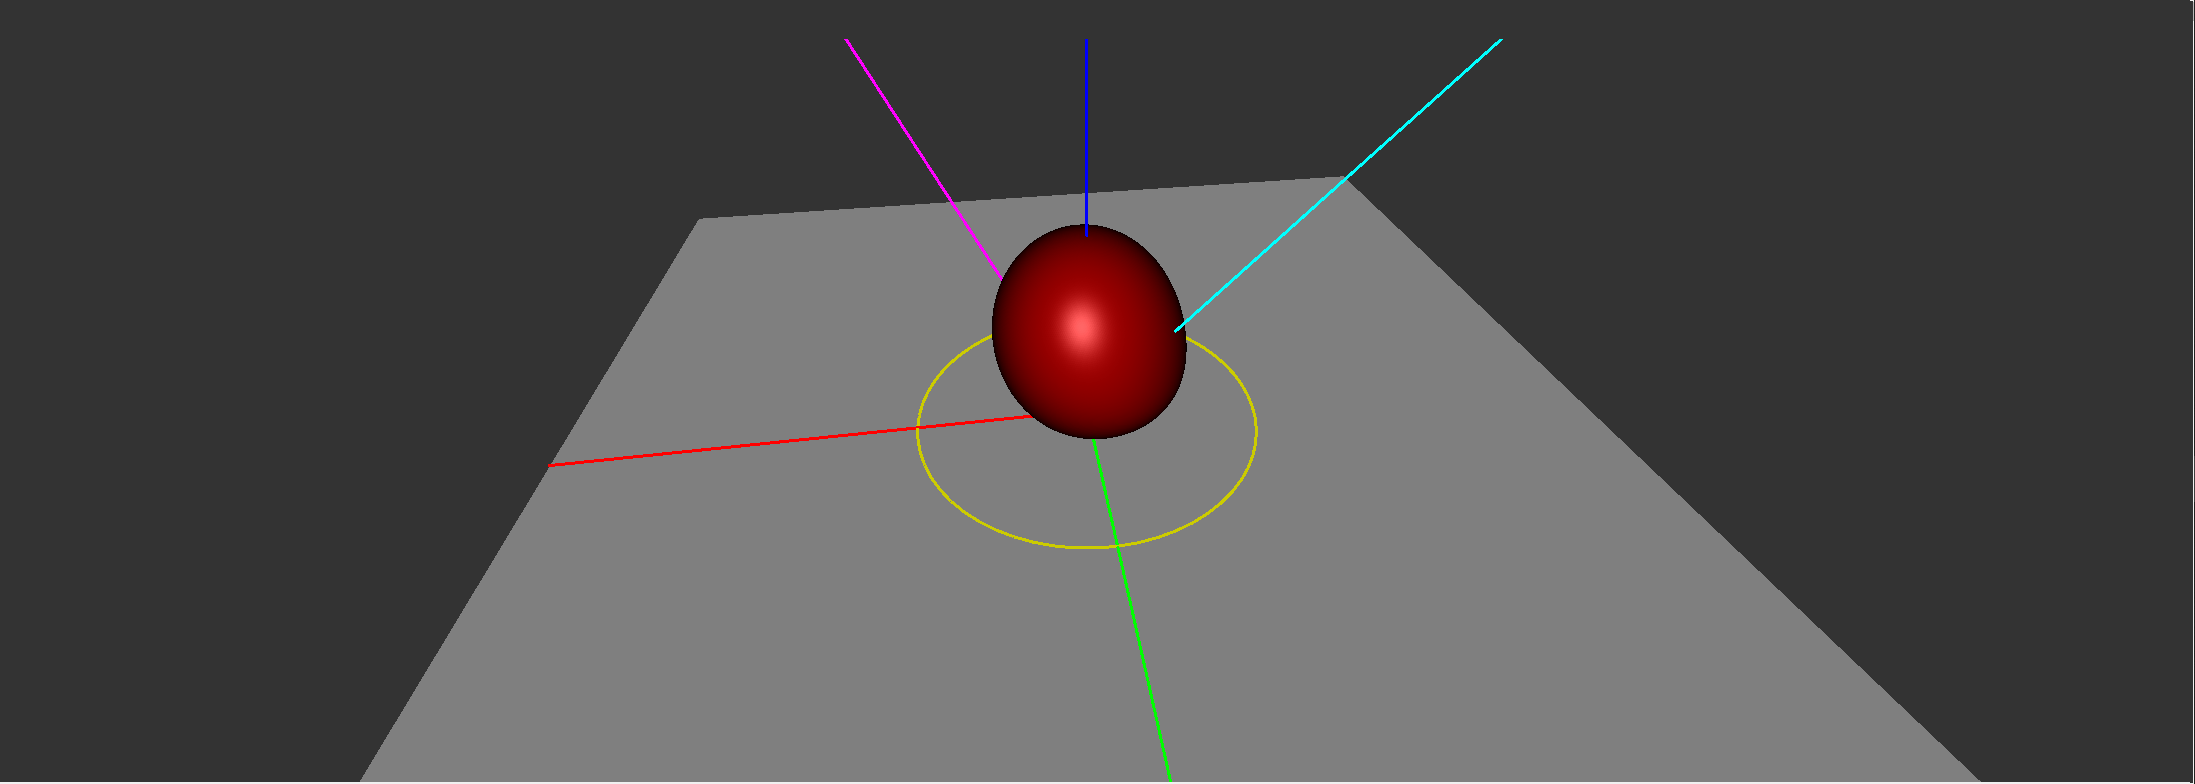
\includegraphics[width=\linewidth]{./Imagens/brdfs/edwards-2006-3D-plot}
    % \caption{\small{(a)}}\label{fig:awesome_image1}
    % \vspace{0.1px}
    % \legend{ \small (a) 3D \textit{plot}}
\endminipage\hfill
\minipage{0.48\textwidth}
  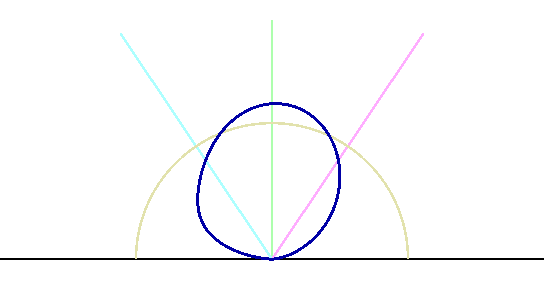
\includegraphics[width=\linewidth]{./Imagens/brdfs/edwards-2006-polar-plot.png}
    % \legend{ \small (b) \textit{Polar plot}}
    % \caption{\small{(b)}}\label{fig:awesome_image1}
\endminipage\hfill
\end{figure}
\end{frame}

\begin{frame}{Experimento Edwards-2006: Objetos 3D renderizados para esta BRDF}
\begin{figure}[H]
    \label{fig-edwards-2006-eqlang}
\minipage{0.32\textwidth}
  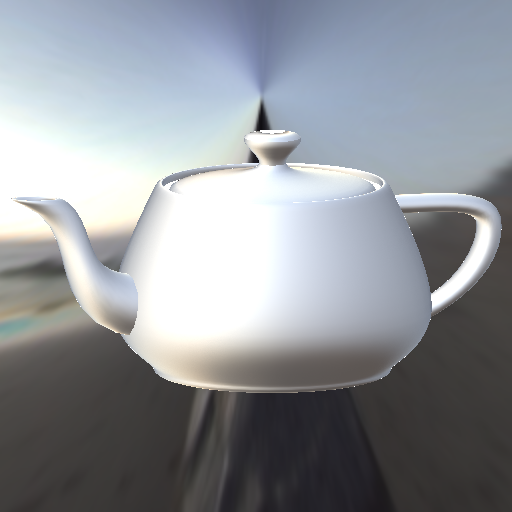
\includegraphics[width=\linewidth]{./Imagens/brdfs/edwards-2006-teapot.png}
    % \legend{ \small (a) \textit{Teapot}}
\endminipage\hfill
\minipage{0.32\textwidth}
  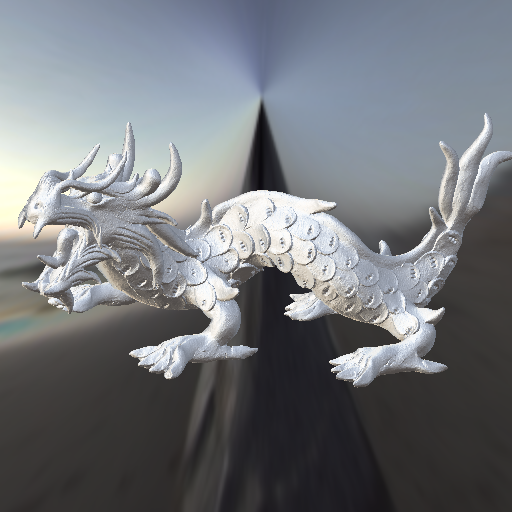
\includegraphics[width=\linewidth]{./Imagens/brdfs/edwards-2006-dragon.png}
    % \legend{ \small (b) Dragão de Stanford}
\endminipage\hfill
\minipage{0.32\textwidth}%
  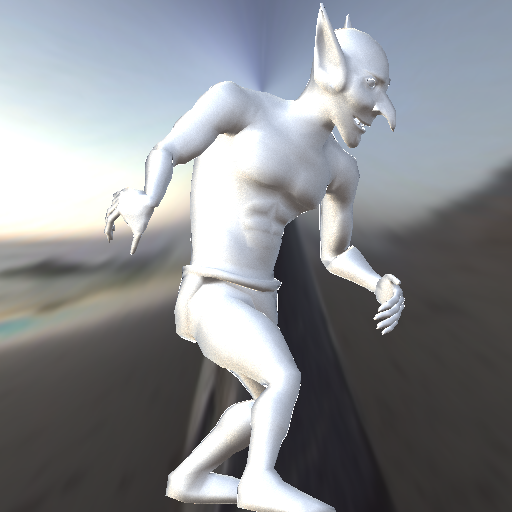
\includegraphics[width=\linewidth]{./Imagens/brdfs/edwards-2006-goblin.png}
    % \legend{ \small (c) Goblin}
\endminipage
\end{figure}
\end{frame}

%%%%%%%%%%%%%%%%%%%%%%%%%%%%%%%%%%%%%%%%%%%%%%%%%
% \subsection{Experimento Edwards-2006}
%%%%%%%%%%%%%%%%%%%%%%%%%%%%%%%%%%%%%%%%%%%%%%%%%


\begin{frame}[fragile]{Resultados: Visão Simplificada dos Outros Experimentos}
   \begin{table}
       \centering
       \scriptsize % Tamanho de texto ajustável (\scriptsize ou \footnotesize)
       \begin{tabular}{|c|c|c|c|c|}
           \hline
           \textbf{Experimento}        & Blinn-Phong     & Cook-Torrance   & Ward           & Ashikhmin-Shirley \\ \hline
           \textbf{Visualização} &
           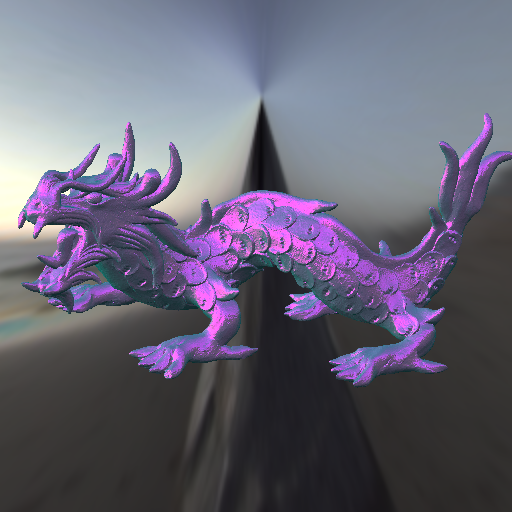
\includegraphics[scale=0.14]{./Imagens/brdfs/blinn-phong-dragon.png} & 
           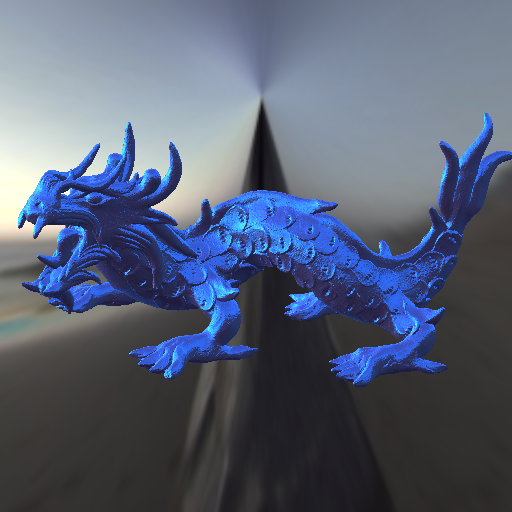
\includegraphics[scale=0.14]{./Imagens/brdfs/cook-torrance-dragon.png} & 
           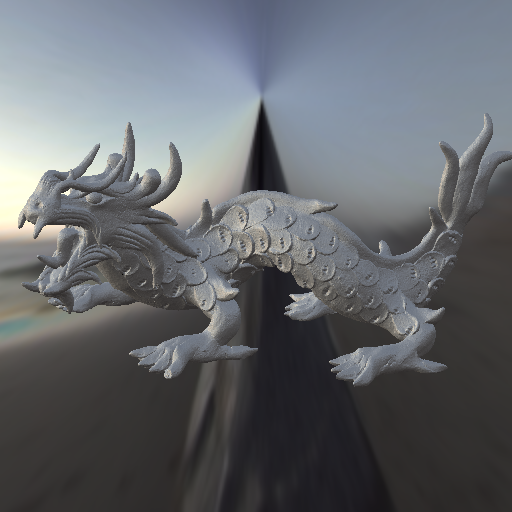
\includegraphics[scale=0.14]{./Imagens/brdfs/ward-dragon.png} & 
           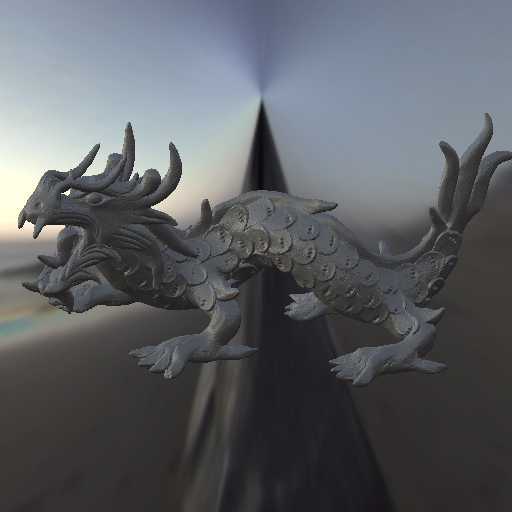
\includegraphics[scale=0.14]{./Imagens/brdfs/ashikhmin-shirley-close-to-original-dragon.png} \\ \hline
       \end{tabular}
   \end{table}

   \begin{table}
       \centering
       \scriptsize % Tamanho de texto ajustável (\scriptsize ou \footnotesize)
       \begin{tabular}{|c|c|c|c|c|}
           \hline
           \textbf{Experimento}        & Oren-Nayar     & Ashikhmin-Shirley$_2$   & Cook-Torrance$_2$ & Dür \\ \hline
           \textbf{Visualização} &
           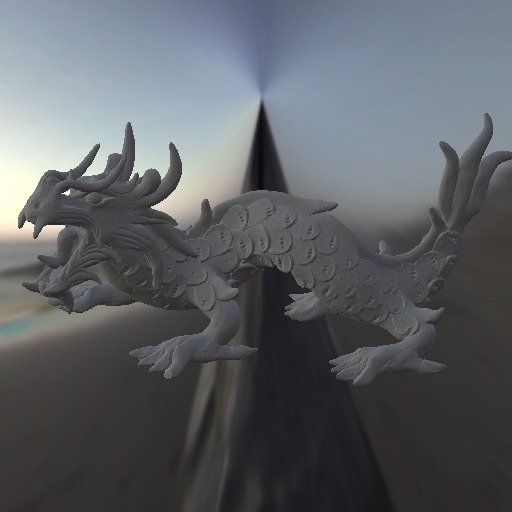
\includegraphics[scale=0.14]{./Imagens/brdfs/oren-nayar-dragon.png} &
           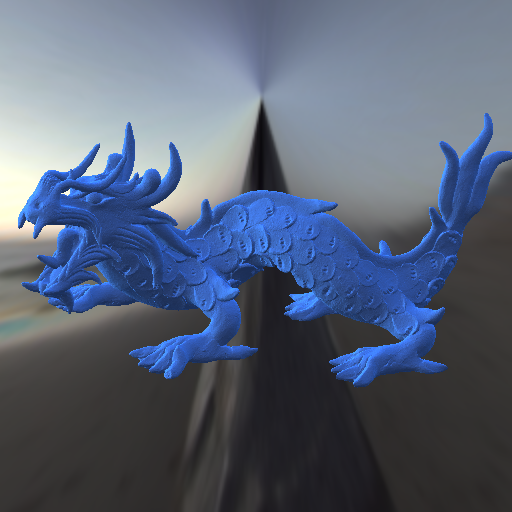
\includegraphics[scale=0.14]{./Imagens/brdfs/ashikhmin-shirley-alternative-dragon.png} &
           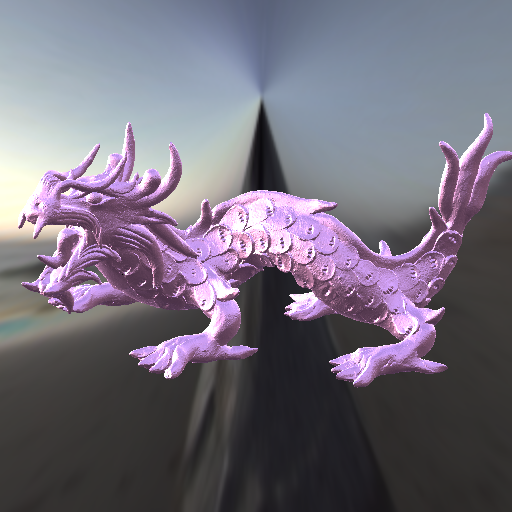
\includegraphics[scale=0.14]{./Imagens/brdfs/cook-torrance-alternative-dragon.png} &
           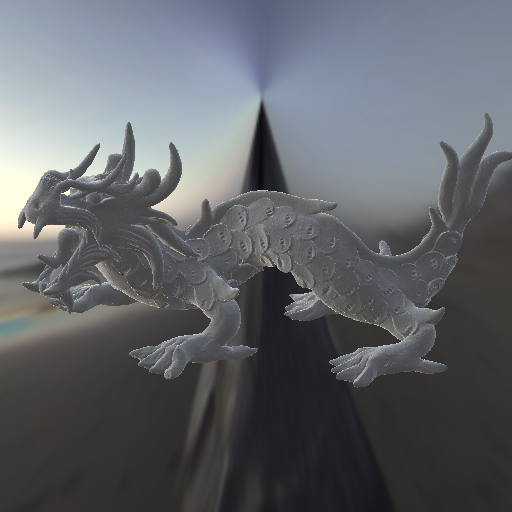
\includegraphics[scale=0.14]{./Imagens/brdfs/duer-dragon.png} \\ \hline
       \end{tabular}
   \end{table}

   \begin{table}
       \centering
       \scriptsize % Tamanho de texto ajustável (\scriptsize ou \footnotesize)
       \begin{tabular}{|c|c|c|c|}
           \hline
           \textbf{Experimento}        & Edwards-2006     & Kajiya-Kay-1989$_*$   & Minnaert \\ \hline
           \textbf{Visualização} &
           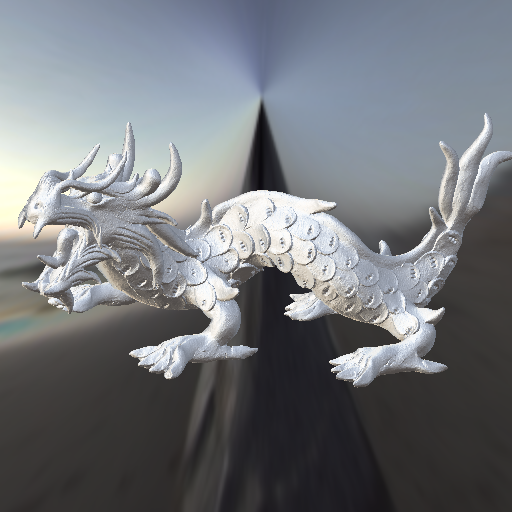
\includegraphics[scale=0.14]{./Imagens/brdfs/edwards-2006-dragon.png} &
           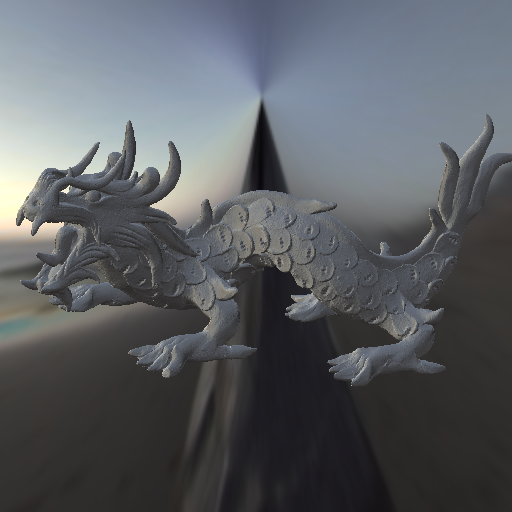
\includegraphics[scale=0.14]{./Imagens/brdfs/aniso-dragon.png} &
           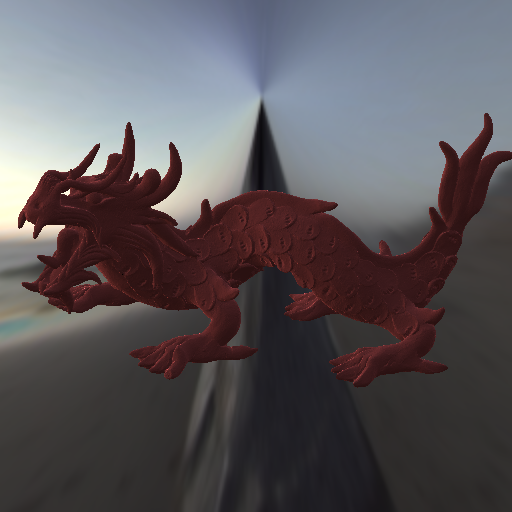
\includegraphics[scale=0.14]{./Imagens/brdfs/minnaert-dragon.png}\\ \hline
       \end{tabular}
   \end{table}
\end{frame}

